\subsection*{Понятие о стрессе}

\note{\hyperlink{growth}{Рост} и \hyperlink{evolution}{развитие} растения происходят под воздействием постоянно меняющихся условий окружающей среды. В ответ на действие неблагоприятных факторов среды растение начинает испытывать стресс}

\paragraph*{}\gls{stress} -- это общая неспецифическая адаптационная реакция организма на действие любых неблагоприятных факторов. 

\paragraph*{}\gls{stressors} -- это неблагоприятные факторы внешней среды, способные вызвать \gls{stress}.  


\paragraph*{}Для растений, как и для других организмов характерны три фазы стресса: 

\begin{enumerate}
	\item Первичная стрессовая реакция;
	\item Фаза адаптации;
	\item Фаза истощения;
\end{enumerate}

\paragraph*{}Действие стрессора зависит от:

\begin{enumerate}
	\item Величины  повреждающего фактора
	\item Длительности его воздействия 
	\item Сопротивляемости растения
	\item Фазы онтогенеза
\end{enumerate}

\paragraph*{}\remember{Наиболее устойчивы растения, находящиеся в состоянии покоя. Наиболее чувствительны растения в молодом возрасте}

\subsubsection*{Первичная стрессовая реакция}

\subsubsection*{Реакция на стресс на клеточном уровне}

\paragraph*{}К первичным неспецифическим процессам, происходящим в клетках растений при действии любых \gls{stressors}ов, относятся:

\begin{enumerate}
	\item Повышение проницаемости мембран, деполяризация мембранного потенциала \hyperlink{plasmolema}{плазмалеммы}.
	\item Вход ионов \hyperlink{calcium}{кальция} в \hyperlink{citoplasma}{цитоплазму} из \hyperlink{cell_wall}{клеточных стенок} и органелл (\hyperlink{cell_vakuol}{вакуоль}, эндоплазматическая сеть, \hyperlink{mitohondria}{митохондрии})
	\item Сдвиг рН цитоплазмы в кислую сторону.
	\item Активация сборки актиновых микрофиламентов цитоскелета, в результате чего возрастает вязкость цитоплазмы.
	\item Усиление поглощения кислорода и траты \gls{atp}, развитие процессов, идущих с образованием свободных радикалов.
	\item Повышение содержания аминокислоты пролина, которая может образовывать гидрофильные коллоиды способствующие удержанию воды в клетке. \note{Пролин может связываться с белковыми молекулами, защищая их от денатурации}
	\item Активация синтеза стрессовых \hyperlink{proteins}{белков}
	\item Усиление активности протонной помпы в \hyperlink{plasmolema}{плазмалемме}, препятствующей неблагоприятным сдвигам в концентрации ионов.
	\item Усиление синтеза \hyperlink{eten}{этилена} и \hyperlink{abscizeAcid}{абсцизовой кислоты}, торможение деления и роста, поглотительной активности клеток.
\end{enumerate}

%\subsubsection*{Специфическое действие стресса на растения}

\subsubsection*{Белки теплового шока}

\paragraph*{}Эти белки локализуются в ядре, цитозоле, клеточных органеллах. 

\paragraph*{}Гены \hypertarget{HeatShockProteins}{белков теплового шока} лишены интронов, а сами белки имеют период жизни около 20 ч, в течение которого клетка сохраняет устойчивость к высокой температуре -- \gls{termoresistens}. 

\paragraph*{}В ядре и ядрышке \gls{HeatShockProteins} образуют гранулы, связывая \gls{dna} и защищая ее тем самым от распада. После прекращения \gls{stress}ового состояния \gls{dna} вновь освобождается и начинают функционировать. 

\paragraph*{}\gls{HeatShockProteins} стабилизируют \hyperlink{plasmolema}{плазмалемму}, проницаемость которой в условиях \gls{stress}а возрастает. 

\subsubsection*{Реакция на стресс на уровне организма}

\paragraph*{}В невысоких дозах повторяющиеся \gls{stress}ы приводят к закаливанию организма, 

\paragraph*{}\remember{Причем закаливание к одному \gls{stressors}у способствует повышению устойчивости организма и другим повреждающим факторам}

\paragraph*{}На уровне организма сохраняются все клеточные механизмы адаптации, а так же начинают проявляться новые механизмы, которые связаны с взаимодействием органов в целом растении. К механизмам адаптации всего растения как целостного организма относятся:

\begin{enumerate}
	\item Конкурентные отношения между отдельными органами за физиологически активные вещества и пищу;

\note{Это позволяет растениям в экстремальных условиях сформировать лишь такой минимум органов, которые они в состоянии обеспечить необходимыми веществами для созревания}

	\item Ускорение процессов старения и опадения нижних листьев и использование продуктов их гидролиза для питания молодых листьев и формирования генеративных органов;

\end{enumerate}

\subsubsection*{Реакция на стресс на уровне популяции}

%Растения способны замещать поврежденные или утраченные органы путем регенерации и роста пазушных почек. Во всех этих процессах коррелятивного роста участвуют межклеточные системы регуляции (гормональная, трофическая и электрофизиологическая).

\paragraph*{}На популяционном уровне включается \hyperlink{naturel_selection_quest}{естественный} отбор, приводящий к появлению более приспособленных к данным условиям организмов и новых видов. 

\paragraph*{}В условиях длительного и сильного \gls{stress}а в первую очередь гибнут неустойчивые растения, тогда, когда более устойчивые, могут выжить и оставить потомство в виде семян. В результате общий уровень устойчивости в популяции возрастает. 

\subsection*{Засухоустойчивость и устойчивость к перегреву} 

\paragraph*{}Действие засухи в первую очередь приводит к уменьшению в клетках свободной воды, что влияет на гидратные оболочки \hyperlink{proteins}{белков} и функционирование \hyperlink{enzimes}{ферментов}

\paragraph*{}При длительном завядании в организме растения происходят следующие изменения: 

\begin{enumerate}
	\item Активируются процессы гидролиза, и, как следствие, увеличивается содержание в клетках низкомолекулярных \hyperlink{proteins}{белков} и \hyperlink{sect_glycosids}{углеводов};
	\item В листьях замедляется синтез \gls{rna} и активируются синтез \hyperlink{ribonukleasa_quest}{рибонуклеаз}; 
	\item В \hyperlink{plasmolema}{цитоплазме} наблюдается распад полисом. 
	\item Изменения \gls{dna}, происходят лишь при длительной засухе;
	\item Из-за уменьшения количества свободной воды возрастает концентрация вакуолярного сока. 
	\item Быстро тормозятся клеточное деление и растяжение, что приводит к образованию мелких клеток и замедлению \gls{growth}а растений. 
	\item Скорость роста корней в начале засухи увеличивается и снижается лишь при длительном недостатке воды в почве. 
	\item При засухе в корнях ускоряется дифференцировка клеток и происходит опробковение и суберинизация экзодермы. 
\end{enumerate}

\paragraph*{}При обезвоживании у растений, не приспособленных к засухе, вначале значительно усиливается, а затем снижается интенсивность \hyperlink{sect_breazing}{дыхания}

\paragraph*{}У засухоустойчивых растений в этих условиях существенных изменений \hyperlink{sect_breazing}{дыхания} не наблюдается.

\paragraph*{}Во время засухи наряду с обезвоживанием происходит еще и перегрев растений. Под действием высокой температуры наблюдается:

\begin{enumerate}
	\item Увеличивается концентрация клеточного сока и проницаемость \hyperlink{plasmolema}{клеточных мембран}.  
	\item В результате выхода из клетки веществ, растворенных в клеточном соке, постепенно снижается осмотическое давление. 
	\item При температуре выше 35 \celsius~ усиливается гидролиз крахмала и белков. Это приводит к увеличению содержания моносахаров, аминокислот и аммиака и, как следствие к повышению осмотического давления.
	\remember{Аммиак токсичен для клеток неустойчивых к перегреву растений}
	\item У жаростойких растений наблюдается рост содержания органических кислот, связывающих избыточный аммиак. 

	\item В клетках растений начинают синтезироваться стрессовые \hyperlink{HeatShockProteins}{белки теплового шока}. 
\end{enumerate}

\paragraph*{}Засухоустойчивость сельскохозяйственных растений повышается в результате предпосевного закаливания семян: 

\note{перед посевом семяна ненадолго намачивания водой, а затем вновь высушивают}

\subsection*{Устойчивость растений к низким температурам}

\paragraph*{}\note{Растения различных мест обитания имеют неодинаковую устойчивость к низким температурам: многие растения Крайнего Севера выдерживают охлаждение до -60 ~\celsius, тогда как большинство теплолюбивых растений южного происхождения плохо переносит низкие положительные температуры. Например, хлопчатник гибнет в течение суток при 1-3 ~\celsius.} 

\paragraph*{}Устойчивость растений к низким температурам подразделяют на:

\begin{enumerate}
	\item \gls{coldResistance} или устойчивость теплолюбивых растений и растений умеренной зоны к низким положительным температурам
	\item \gls{frostResistance} или способность растений переносить температуру ниже 0 \celsius.
\end{enumerate}

\paragraph*{}У теплолюбивых растений при низких положительных температурах:

\begin{enumerate}
	\item \gls{turgor} клеток надземной части резко уменьшается, так как нарушается доставка воды;
	\item Усиливается распад белков и накопление в тканях растворимых форм азота. 
	\item Изменяется функциональная активность \hyperlink{plasmolema}{мембран} из-за перехода липидов из жидкокристаллического состояния в состояние геля.
\end{enumerate}

\paragraph*{}\gls{coldResistance} сельскохозяйственных культур можно усилить внесением калийных удобрений и  предпосевным закаливанием семян. 

\note{Наклюнувшиеся семена теплолюбивых культур (огурцы, томаты, дыня и др.) в течение нескольких суток выдерживают в чередующихся через 12 часов условиях низких (1-5 \celsius) и более высоких (10-20 \celsius) температур. Таким же способом можно затем закаливать рассаду}

\paragraph*{}\gls{coldResistance} повышается при замачивании семян в 0,25 \% растворах микроэлементов или нитрата аммония.

\paragraph*{}Под воздействием отрицательных температур клетки растения гибнут в основном из за их обезвоживания и повреждения клеточных структур растущими кристаллами льда. Обезвоживание возникает из-за того, что растущие в межклетниках кристаллы льда оттягивают на себя воду из цитоплазмы клеток. При длительном действии мороза кристаллы льда вырастают до значительных размеров и могут повреждать плазмалемму.

\paragraph*{}Среди приспособлений, позволяющих морозостойким растениям вынести низкие температуры можно выделить следующие:

\begin{enumerate}
	\item Повышено содержание ненасыщенных жирных кислот в клеточных мембранах. \note{Поэтому фазовый переход липидов мембран из жидкокристаллического состояния в гель происходит при отрицательных температурах}
	\item В состоянии геля резко снижается проницаемость мембран. 
	\item Активно синтезируются \gls{crioprotectors} гидрофильных белков, моно- и олигосахаров. 
	\note{Вода, входящая в состав гидратных оболочек этих веществ, не замерзает и не выходит из клеток}

\end{enumerate}



\subsection*{Закаливание растений}

\paragraph*{}\remember{Закаливание -- обратимое физиологическое приспособление к неблагоприятным воздействиям, происходящее под влиянием определенных внешних условий}

%\note{Физиологическая природа процесса закаливания к отрицательным температурам была раскрыта благодаря работам И.И. Туманова и его школы}

\paragraph*{}В результате процесса закаливания морозоустойчивость организма резко повышается. 


\paragraph*{}Способность растения к закаливанию зависит от таких факторов, как:

\begin{enumerate}
	\item Вид растения;
	\item Его происхождение;
	\note{Растения южного происхождения к закаливанию не способны. У растений северных широт процесс закаливания может происходить лишь на определенном этапе \hyperlink{plant_ontogenesis}{развития}}

\end{enumerate}

\paragraph*{}Для приобретения способности к закаливанию растения должны закончить процессы роста, должен завершится отток веществ. 

\remember{Сигналом к прекращению \gls{growth}а и стимулом для изменений в гормональной системе для растений является сокращение фотопериода и снижение температуры}
%Ослабляется синтез ИУК и гиббереллинов, усиливается образование АБК и этилена –> рост простанавливается.

\paragraph*{}\note{Если в течение лета у древесных растений процессы роста не успели закончиться, то это может вызвать массовую гибель растений зимой. Так, зимняя гибель часто вызывается летней засухой. Засуха приостанавливает рост летом и не позволяет древесным культурам завершить ростовые процессы к осени. В результате растения оказываются неспособными пройти процессы закаливания и гибнут даже при небольших морозах}
%Аналогичная картина характерна для растений, выращенных при несоответствующем фотопериоде, не успевших завершить летний рост и поэтому неспособных к закаливанию. 

\paragraph*{}Способность к закаливанию утрачивается весной в связи с началом \gls{growth}а растения. 

\note{К закаливанию способен лишь целостный организм, при обязательном наличии корневой системы. Клетки корня вырабатывают вещества, повышающие устойчивость организма против мороза}

\paragraph*{}Собственно процесс закаливания требует комплекса внешних условий и проходит в две фазы.

\subsubsection*{Первая фаза закаливани}

\paragraph*{}Первая фаза закаливания проходит при следующих условиях

\begin{enumerate}
	\item На свету. Свет в процессе закаливания оказывает регуляторное влияние на генетический аппарат клетки и способствует активизации генов, участвующих в переходе в покоящееся состояние;
	\item При несколько пониженных плюсовых температурах; \note{Так, защитное действие сахаров проявляется только в том случае, если происходит при одновременном понижении температуры}
	\item При умеренной влажности; \note{Излишняя влажность почвы (дождливая осень) препятствует прохождению процесса закаливания}
\end{enumerate}

\paragraph*{}В эту фазу продолжается замедление ростовых процессов вплоть до их полного прекращения. В растении накапливаются вещества-\gls{crioprotectors}, выполняющих защитную функцию. Криопротекторами являются:

\begin{enumerate}
	\item Сахароза;
	\item Моносахариды;
	\item Растворимые белки;
\end{enumerate}

%В этих условиях образование сахаров в процессе фотосинтеза идет с достаточной интенсивностью. 
%Более морозостойкие виды и сорта характеризуются большей способностью к накоплению сахаров именно при пониженной температуре. 
\paragraph*{}Эти вещества локализуются в разных частях клетки: клеточном соке, цитоплазме, органеллах. 

\paragraph*{Роль сахаров в повышении устойчивости растений к низким температурам}: 

\begin{enumerate}
	\item Сахара повышают концентрацию клеточного сока, снижают водный потенциал. 
	\note{Как вам уже известно из курса химии, чем выше концентрация раствора, тем ниже его точка замерзания}%Привести задачу на расчет температуры замерзания
	\item Сахара повышают устойчивость специфических белков, образующихся при пониженной температуре. 
\end{enumerate}

\paragraph*{}Кроме вышеназванных процессов, в первый период закаливания происходит:

\begin{enumerate}
\item Уменьшение содержания свободной воды. 
\note{Чем меньше в клетках и тканях содержание воды, тем меньше образуется льда и тем меньше опасность повреждения}
\item В составе мембран возрастает уровень и изменяется структура фосфолипидов
\item Повышается содержание ненасыщенных жирных кислот. Это позволяет поддерживать высокую проницаемость мембран, необходимую для транспорта воды. 
\item Происходит перестройка ферментных систем процесса дыхания, возрастает альтернативный путь дыхания

\end{enumerate}

\paragraph*{Белки холодового шока}

%Ряд стрессовых белков, к которым относят десатуразы, дегидрины — LEA-белки, 
\paragraph*{}\gls{frostShockProteins} -- эти гидрофильные белки синтезируются в цитоплазме под действием низких температур и выделяются в клеточную стенку. 
\paragraph*{}\gls{frostShockProteins} выполняют в клетке следующие функции:

\begin{enumerate}
\item Располагаются на поверхности кристаллов льда, препятствуют их росту
\item Разобщают окислительное фосфорилирование, что позволяет использовать энергию окисления на повышение температуры органов растений на 4-7~ \celsius~ выше окружающего воздуха.
\end{enumerate} 



%В последние годы были изолированы гены, ответственные за синтез БХШ, образование которых позволяет переносить низкие температуры. В арабидопсисе идентифицирован ген — гомолог «противоморозного» гена, от которого зависит способность адаптироваться к низким температурам. Показана роль АБК в образовании этих белков. Так, мутанты арабидопсиса, не способные к синтезу АБК, не обладают устойчивостью к низким температурам. Значение АБК подтверждается тем, что при низких температурах возрастание содержания АБК в растении увеличивает и устойчивость. Например, проростки люцерны переносят температуру до —10°С. Это свойство может быть увеличено путем предварительного выдерживания при 4°С или обработкой АБК, поскольку оба эти способа вызывают синтез БХШ. 

\paragraph*{}К концу первой фазы закаливания клетки растений переходят в покоящееся состояние. Цитоплазма обособляется от \hyperlink{cell_wall}{клеточной стенки}, что, в свою очередь, снижает возможность повреждения цитоплазмы образующимися в межклетниках кристаллами льда. Особенно интенсивно перестройка обмена веществ происходит в период второй фазы закаливания.

\subsubsection*{Вторая фаза закаливания}

\begin{enumerate}
	\item Начинается при дальнейшем понижении температуры (около 0 \celsius);
	\item Не требует света;
	\note{Для травянистых растений она может протекать и под снегом}
\end{enumerate} 
 
\paragraph*{}В эту фазу происходит 

\begin{enumerate}
	\item Отток воды из клеток;
	\item Перестройка структуры протопласта;
	\item Продолжается новообразование специфических, устойчивых к обезвоживанию белков;
\end{enumerate}

\paragraph*{Перестройка структуры протопласта}

\paragraph*{}Из за того, что ввода оттягивается из цитоплазмы растущими в межклетниках кристаллах льда, происходит обезвоживание клетки и сближение белков протопласта. Связи между белками разрываются и не восстанавливаются в прежнем виде из-за слишком сильного сближения и деформации белковых молекул. 

\paragraph*{}Вероятность разрушения белков уменьшает наличие  в составе белковой молекулы сульфгидрильных и других гидрофильных группировок, которые способствуют удержанию воды и препятствуют сближению молекул белка. 

\remember{Перестройка цитоплазмы способствует увеличению ее проницаемости для воды. Благодаря более быстрому оттоку воды уменьшается опасность образования льда внутри клетки}

%Не для всех растений необходимо протекание процессов закалива­ния в две фазы. У древесных растений, обладающих достаточным количеством Сахаров, сразу протекают изменения, соответствующие второй. 

\paragraph*{}Таким образом, в процессе закаливания возникает \gls{frostResistance}, которая определяется рядом изменений: 

\begin{enumerate}
\item У закаленных растений благодаря высо­кой концентрации клеточного сока, уменьшению содержания воды кристаллы льда образуются не в клетке, а в межклетниках.
\item Значительно уменьшается количество образовавшегося в межклетниках льда
\item Изменение свойств белков цитоплазмы делает их более устойчивыми к обезвоживанию. 
\item Накопление сахаров оказывает дополнительное защитное влияние. Важное значение имеет повышение устойчивости мембран к обезвоживанию и механическому давлению.
\end{enumerate}
 
%Имеются данные, что при закаливании увеличивается количество фосфолипидов и ненасыщенных жирных кислот. Важно отметить, что в клетках закаленных растений накапли­вается АТФ. Чем больше развитие указанных признаков у отдельных видов и сортов растений, тем выше их морозоустойчивость. 
\paragraph*{}\gls{frostResistance} -- комплексный признак, запрограммированный генетически, однако он проявляется в определенных условиях среды. Повышение температуры весной сопровожда­ется противоположными изменениями. Поэтому весной растения часто гибнут даже от небольших заморозков. 

\note{Усиление фосфорного питания повы­шает устойчивость растений к морозу, тогда как азотные удобрения, способст­вуя процессам роста, делают растения более чувствительными}
%Благоприятное влияние на морозоустойчивость оказывает обработка такими микроэлементами как цинк, молибден, кобальт. Очень большое значение имеет также выведение морозоустойчивых сортов растений. Делаются попытки создания морозо­устойчивых трансгенных растений путем введения генов, кодирующих ферменты синтеза веществ-криопротекторов, например, пролина и бетаина.

\subsection*{Солеустойчивость}

\paragraph*{}Растения, устойчивые к засолению, называют \gls{gallophites}. Растения же незасоленных водоемов и почв носят название \gls{glycophites}. У гликофитов при засолении снижается рост клеток растяжением, нарушается азотный обмен и накапливается токсичный аммиак.

\paragraph*{}Все галофиты делят на три группы:

\begin{enumerate}
	\item Настоящие галофиты (эугалофиты) - наиболее устойчивые растения, накапливающие в вакуолях значительные количество солей. Поэтому они обладают большой сосущей силой, позволяющей поглощать воду из сильно засоленной почвы. Для растений этой группы характерна мясистость листьев, которая исчезает при выращивании их на незасоленных почвах.
	\item Солевыделяющие галофиты (криногалофиты), поглощая соли, не накапливают их внутри тканей, а выводят из клеток на поверхность листьев с помощью секреторных железок. Выделение солей железками осуществляется с помощью ионных насосов и сопровождается транспортом больших количеств воды. Соли удаляется с опадающими листьями. У некоторых растений избавление от избытка солей происходит без поглощения больших количеств воды, так как соль выделяется в вакуоль клетки-головки листового волоска с последующим ее обламыванием и восстановлением.
	\item Соленепроницаемые галофиты (гликогалофиты) растут на менее засоленных почвах. Высокое осмотическое давление в их клетках поддерживается за счет продуктов фотосинтеза, а клетки малопроницаемы для солей. 
\end{enumerate}

\paragraph*{}Солеустойчивость растений увеличивается после предпосевного закаливания семян. 
\begin{enumerate}
\item Для повышения устойчивости к хлоридному засолению семяна замачивают один час в 3 \% растворе NaCl с последующим промыванием водой в течение 1,5 часа
\item Для повышения устойчивости к сульфатному засолению семена в течение суток вымачивают в 0,2 \%-ном растворе сульфата магния
\end{enumerate}

\subsection*{Устойчивость к недостатку кислорода}

\paragraph*{}Кислородная недостаточность (\gls{gipoxia}) возникает при следующих условиях: 
\begin{enumerate}
\item Временном или постоянном переувлажнении;
\item При заболачивании почвы;
\item При образовании ледяной корки на озимых посевах и хранении сельскохозяйственной продукции;
\end{enumerate}

\paragraph*{}У растений могут присутствовать следующие приспособления предотвращающие гипоксию:

\begin{enumerate}
\item У растений, корни которых постоянно испытывают недостаток кислорода происходит разрастание основания стебля, образование дополнительной поверхностной корневой системы и вентиляционных систем межклетников, необходимых для транспорта кислорода из надземной части растения в корни (\ris \ref{anti_gipoxia})
\item У некоторых растений активируется пентозофосфатный и гликолитический пути дыхания.
\item В устойчивых к кислородному дефициту растениях не накапливаются токсичные продукты анаэробного распада.
\item \gls{anoxicOxigenation}, в ходе которого электроны переносятся на нитраты и двойные связи ненасыщенных соединений;
\end{enumerate}

%%%%%%%%%%%%%%%%%%%%%%%%%%%%%%%%%%%%%%%%%%%%%%%%%%%%%%%%%%%%%%%%%%%%%%%%%%%%%%%%%%%%%%%%%%%%%%%%%%%%%%%

\begin{figure}[h]
\begin{minipage}[h]{0.49\linewidth}
\center{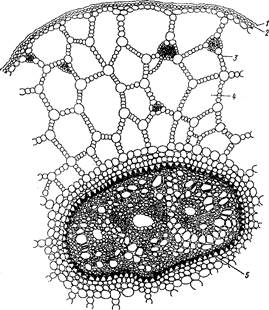
\includegraphics[width=0.8\linewidth]{pictures/aerenchima} \\ а) \gls{aerenhima} рдеста}
\end{minipage}
\hfill
\begin{minipage}[h]{0.49\linewidth}
\center{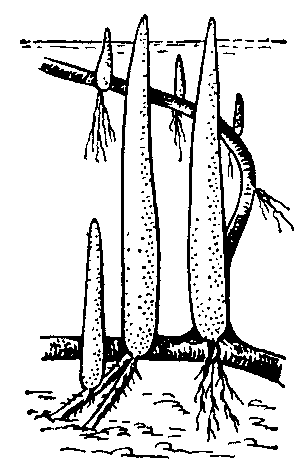
\includegraphics[width=0.8\linewidth]{pictures/pnevmatofory} \\ б) \gls{pneumatophores} мангровых деревьев \cite{gilarow}}
\end{minipage}
\caption{Приспособление растений к недостатку кислорода}
\label{anti_gipoxia}
\end{figure}

%%%%%%%%%%%%%%%%%%%%%%%%%%%%%%%%%%%%%%%%%%%%%%%%%%%%%%%%%%%%%%%%%%%%%%%%%%%%%%
\note{Для повышения устойчивости к гипоксии замачивают семена в растворах хлорхолинхлорида, никотиновой кислоты или сульфата марганца}

\subsection*{Газоустойчивость}

\paragraph*{}\gls{gassResistance} -- способность растений сохранять жизнедеятельность при действии вредных газов. Токсичные газы, попадая в листья, образуют кислоты или щелочи. Это приводит к: 

\begin{enumerate}
	\item Изменению рН цитоплазмы;
	\item Разрушению хлорофилла;
	\item Нарушению клеточных мембран;
\end{enumerate}

\paragraph*{}Для разных видов растений характерен свой безопасный для жизнедеятельности уровень накопления токсичных газов. 

\note{Так, лох, тополь и клен более устойчивы к хлору и сернистому газу ($SO_{2}$), чем липа и каштан}

\paragraph*{}Растения, устойчивые к засолению и другим стрессорам, имеют более высокую газоустойчивость.

\paragraph*{}\gls{gassResistance} растений повышается при оптимизации минерального питания и водоснабжения, а также в результате закаливания семян. 

\note{Замачивание семян в слабых растворах соляной и серной кислот повышает устойчивость растений к кислым газам}

\subsection*{Радиоустойчивость}

%Различают прямое и косвенное действие радиации на живые организмы. 
\paragraph*{}Прямое действие энергии излучения на молекулу переводит ее в возбужденное или ионизированное состояние. Особенно опасны повреждения структуры ДНК:

\begin{enumerate}
\item Разрывы связей сахар-фосфат;
\item Дезаминирование азотистых оснований;
\item Образование димеров пиримидиновых оснований;
\end{enumerate}

\paragraph*{}Косвенное действие радиации заключается в повреждениях молекул, продуктами радиолиза воды. Заряженная частица излучения, взаимодействуя с молекулой воды, вызывают ее ионизацию. Ионы воды способны образовать химически активные свободные радикалы и пероксиды. Эти сильные окислители могут повредить нуклеиновые кислоты, белки-ферменты, липиды мембран.
%Ионы воды за время жизни 10-15 - 10-10 сек способны образовать химически активные свободные радикалы и пероксиды. Эти сильные окислители за время жизни 10-6 - 10-5 сек могут повредить нуклеиновые кислоты, белки-ферменты, липиды мембран. 
%Первоначальные повреждения усиливаются при накоплении ошибок в процессах репликации \gls{dna}, синтеза \gls{dna} и белков.

\paragraph*{}Устойчивость растений к действию радиации определяется следующими факторами:

\begin{enumerate}

	\item Постоянным присутствием ферментных систем восстановления (\gls{reparation} \gls{dna}). При контакте с поврежденным участком \gls{dna}, ферменты репарции разрушают его, а затем восстанавливают целостность молекулы \gls{dna}. 
	\item Наличием в клетках веществ-радиопротекторов \note{сульфгидрильные соединения, аскорбиновая кислота, каталаза, пероксидаза, полифенолоксидаза}. \gls{radioprotectors} нейтрализуют свободные радикалы и пероксиды, возникающие при облучении.
	\item Действием механизмов, обеспечивающих восстановления всего организма: 

	\begin{enumerate}
		\item Неоднородностью популяции делящихся клеток меристем, которые содержат клетки на разных фазах \hyperlink{cellCycle}{митотического цикла} с неодинаковой радиоустойчивостью;
		\item Присутствием в апикальных меристемах покоящихся клеток, которые приступают к делению при остановке деления клеток основной меристемы;
		\item Наличием спящих почек, которые после гибели апикальных меристем начинают активно функционировать и восстанавливают повреждение;

	\end{enumerate}

\end{enumerate}

\subsection*{Устойчивость растений к биотическим факторам}

\paragraph*{}\remember{Устойчивость к инфекции -- это способность растения предотвращать, ограничивать и задерживать ее развитие} 
%Основоположник учения об устойчивости растений Н. И. Вавилов выделял устойчивость 

\paragraph*{}Выделяют следующие виды устойчивости:

\begin{enumerate}
	\item Неспецифическую (видовую) или фитоиммунитет;
	\item Специфическую (сортовую)
\end{enumerate}

\subsubsection*{Фитоиммунитет}

\paragraph*{}Фитоиммунитет представляет собой полную невосприимчивость (возбудитель не поражает данный вид растения). 

\note{Например, бобовые не поражаются болезнями пасленовых} \paragraph*{}Неспецифический иммунитет защищает растения и от множества \gls{saprotroph}ных организмов, в окружении которых они постоянно находятся. Благодаря данному типу иммунитета растения поражаются лишь небольшим числом возбудителей. 

\remember{В процессе эволюции некоторые \gls{patogen}ы сумели преодолеть видовой иммунитет и стали паразитами, специфичными для этого вида. На такие \gls{patogen}ы приходится 90\% потерь урожая сельскохозяйственных культур}
%Белковые продукты генов устойчивости полифункциональны, а сами эти гены имеют разное происхождение. 
\paragraph*{}Гены устойчивости происходят от генов, кодировавших необходимые для развития белки, участвующие в эндогенных сигнальных системах. Для растений характерен специфичный механизм быстрой эволюции генов устойчивости, отсутствующий у животных, которые имеют развитую соматическую иммунную систему.
%Например, растения риса (Oryza sativa) для обнаружения \gls{patogen}а мобилизуют белки, определяющие межклеточные связи с участием внеклеточного компонента. Некоторые белки, связанные с инициацией защитного отклика, подобны белкам, вызывающим запрограммированную смерть клетки.
 
%У растений зафиксировано появление устойчивости ко второму возбудителю после предшествующей инфекции или ослабление устойчивости к патогену при заболевании, вызванном другим возбудителем.

\subsubsection*{Механизмы защиты от патогенов и теории устойчивости}

\paragraph*{}Общая стратегия защиты растения от \gls{patogen}ов -- не допустить со действие патогена на клетки, локализовать инфекцию и уничтожить патоген.

\paragraph*{}Есть несколько \hyperlink{resistence_theories_quest}{теорий}, объясняющих причины устойчивости растений к определенным \gls{patogen}ам:

\begin{enumerate}

	\item Хемотропичная теория: растения могут поражаться определенным патогеном, если содержат привлекающие паразитов вещества, диффундирующие через клеточную стенку, а если таких веществ нет, то растение устойчиво. \note{Однако было показано, что споры грибов могут прорастать не только через живую ткань, но и через клетки эпидермиса, лишенные содержимого как у восприимчивых, так и у устойчивых растений. Заражение же зависит от процессов, развивающихся при взаимодействии продуктов патогена с мембраной клетки}
	\item Тормозящая теория: устойчивые растения содержат вещества, тормозящие развитие патогена. 
	\item Питательная теория (теория <<неполной среды>>) связывает устойчивость растения с отсутствием в нем необходимых паразиту веществ.

\end{enumerate}


\paragraph*{}Защита растений от патогенов -- это комплексное явление, включающее два вида механизмов: 

\begin{enumerate}
	\item Конституционные, которые присутствуют в организме растения еще до его контакта с патогеном;
	\item Индуцированные, которые возникают в ответ на контакт с паразитом или с его выделениями;
\end{enumerate}

\paragraph*{}Конституционные механизмы включают: 

\begin{enumerate}
	\item особенности клеток и тканей, обеспечивающие механический барьер для проникновения инфекции;
	\item способность выделять антибиотические вещества; 
	\item создание в тканях недостатка важных веществ для роста и развития паразита. 
\end{enumerate}

\paragraph*{}Индуцированные механизмы устойчивости к инфекции растение проявляет через:

\begin{enumerate}
	\item Усиление дыхания и энергетического обмена;
	\item Накопление веществ, обеспечивающих общую неспецифическую устойчивость (фитонциды, фенолы и продукты их окисления); 
	\item Создание дополнительных механических барьеров; 
	\item Возникновение реакции сверхчувствительности; 
	\item Быстрый синтез низкомолекулярных защитных веществ -- фитоалексинов.
\end{enumerate}

\paragraph*{}Устойчивость растений к воздействию \gls{biotroph}ов поддерживается при помощи: 

\begin{enumerate}
	\item Механизмов распознавания паразита; 
	\item Включения реакции сверхчувствительности и последующего уничтожения патогена в некрозной зоне с участием синтезированных в ответ на инфекцию фитоалексинов;
\end{enumerate}

\paragraph*{}Устойчивость же к \gls{necrotroph}ам обеспечивается с помощью: 

\begin{enumerate}
\item Способности обезвреживать токсины паразита;
\item Потери устойчивыми растениями чувствительности к специализированным токсинам; 
\item Присутствия на \hyperlink{plasmolema}{мембране} клетки хозяина рецептора, связывающего токсин; 
\item Инактивации экзоферментов неспецифическими ингибиторами; 
\item Задержки синтеза экзоферментов паразита устранением или маскировкой субстратов
\remember{\gls{exoenzims} -- ферменты, выделяемые растениями во внешнюю среду}
\note{например, усиление суберинизации и лигнификации клеточных стенок в месте поранения маскирует пектиновые вещества, необходимые для начала синтеза пектиназ паразита} 
\item Повреждения клеточных стенок паразита ферментами растения (хитиназой, глюконазой); 
\item Синтеза белков-антиферментов в ответ на гидролитические ферменты паразита \cite{polevoy_89}.
\end{enumerate}

\paragraph*{}Взаимодействие с паразитом начинается на поверхности растения. Патоген или его споры должны сначала удержаться на ней, а потом проникнуть в растительную клетку Препятствовать этому может ряд механических барьеров: 

\begin{enumerate}
\item Создания на поверхности эпидермы воскового слоя, делающего эпидерму гладкой и плохо смачиваемой водой, необходимой для прорастания спор. 
\note{Патоген может преодолеть этот барьер, проникнув внутрь растения через устьица, чечевички и раны. Грибы, кроме того, могут разрушать кутикулу своими выделениями}
\item Покровные ткани могут содержать в своем составе антибиотики;
\item Усиленное одревеснение (лигнификация) клеток;
\note{Лигнификация повышает механическую прочность клеточных стенок, ограничивает распространение токсинов паразита и приток питания к нему, защищает стенку клетки от действия ферментов паразита. Лигнифицироваться может и клеточная стенка грибов-паразитов, что останавливает их рост \cite{polevoy_89}.}
\item Механической преградой для патогенов, распространяющихся по сосудам растения, становятся образующиеся в них \gls{tiles} -- покрытые пектиновым чехлом выпячивания содержимого соседних паренхимных клеток;
\end{enumerate}

\subsubsection*{Питательная теория}

\paragraph*{}Питательная теория (теория <<неполной среды>>) объясняет устойчивость растения к патогенам отсутствием в нем необходимых паразиту веществ. Паразит в процессе эволюции так приспосабливается к обитанию внутри своего хозяина, что со временем утрачивает способность к самостоятельному синтезу различных необходимых ему веществ. Эти вещества он берет из клеток своего хозяина.
%Она опирается на работы по мутантным грибам, неспособным самостоятельно синтезировать необходимые для роста и развития вещества. Такие грибы не поражают растения, которые не содержат данных веществ, но при искусственном введении их устойчивость растения к паразиту теряется.
%Например питательная теория объясняет взаимодействия растений с зависимыми от них высокоспециализированными биотрофами. 
\note{Примером может быть устойчивость пшеницы к фузариозу. Растение теряет устойчивость к грибу Fusarium graminearum во время цветения, так как заражение происходит через пыльники, в которых содержатся азотсодержащие метилированные спирты, входящие в состав его фосфолипидов. Экспериментальное добавление этих веществ усиливает инфекционность гриба, но не влияет на другие патогены, не нуждающиеся в них. И в целом круг растений, поражаемых этим грибом, ограничен видами, содержащими высокие концентрации данных спиртов} 

%Реже питательной теорией можно объяснить сортовую устойчивость. Так, некоторые сорта риса (Oryza sativa) устойчивы к Xanthomonas oryzae. Эта бактерия зависит от наличия в среде аминокислот, содержащих серу, так как не может использовать неорганические ее источники. Добавление выделенного из злака цистеина стимулирует рост паразита и повышает его патогенность. Поэтому сорта, не содержащие этого вещества (или бедные им), устойчивы к данной бактерии (J1. Г. Косулина и др., 1993).
\paragraph*{}Формирование <<неполной среды>> может происходить в ответ на заражение. При этом растение исключает из обмена необходимые паразиту вещества. 
%Так, К. Т. Сухоруков (1952) показал, что при поражении проводящей системы хлопчатника (Gossypium) возбудителем вилта Verticillium в тканях устойчивых сортов понижается содержание биотина и пантотеновой кислоты. Таким образом, устойчивые растения в отличие от неустойчивых устраняют из очага поражения необходимые грибу вещества, создавая неблагоприятную среду для его роста.
\note{Например, установлено, что устойчивые к фитофторозу сорта картофеля лишают патоген стеринов, которые тот получает из клеток картофеля. $\beta$-ситостерин необходим фитофторе для образования зооспор. У устойчивых растений на инфицированном участке он перестает синтезироваться, так как его предшественник быстро потребляется для начавшегося синтеза защитных веществ \cite{metlitskiy_2013}}

\subsubsection*{Фитонциды}

\paragraph*{}Важную роль в неспецифической защите растений от патогенов играют вырабатываемые растениями антибиотические вещества -- \gls{fitoncides}. Внутри клеток фитонциды часто накапливаются в вакуолях. 

\paragraph*{}Летучие \gls{fitoncides}, выделяемые при повреждении клеток, защищают растения от патогенов уже над поверхностью органа. \note{Например у лука и чеснока} 

\paragraph*{}Нелетучие фитонциды содержатся в покровных тканях, и защищают от патогена поверхность листьев, стеблей и.т.д. После повреждения растений их содержание резко возрастает, предотвращая инфицирование раны. 

\remember{\hyperlink{pests_question}{Специализированные} паразиты довольно легко приспосабливаются к антибиотическим веществам растения хозяина, но роль фитонцидов в неспецифическом фитоиммунитете достаточно велика}

\paragraph*{}С химической точки зрения фитонциды -- это низкомолекулярные вещества разных групп. Среди них наиболее распространены: 

\begin{enumerate}
\item Терпеноиды;
\item Алкалоиды;
\item Эфирные масла;
\item Пигменты;
\item Глюкозиды;
\item Фенольные соединения;
\end{enumerate}
 
\paragraph*{}Защитные свойства многих фитонцидов появляются при их химических превращениях. 

\note{Например, при выходе из состояния покоя в луковицах лука активируется фермент аллииназа, под влиянием которого основной компонент эфирных масел лука аллиин превращается в фитонцид аллицин, обладающий фунгицидным действием. При повреждении патогеном окрашенных органов растений антоциановые пигменты распадаются с образованием токсичного для микроорганизмов антоцианидина}

\paragraph*{}В поврежденных и инфицированных клетках активируются процессы, приводящие к накоплению фенольных соединений \cite{kosulina_93}. Значение фенолов для растения заключается в том, что они

\begin{enumerate}
	\item Инактивируют ферменты, находящиеся на поверхности \gls{patogen}ов; 
	\item Ограничивают диффузию токсинов и питательных веществ, поступающих к \gls{patogen}у; 
	\item Придают прочность механическим тканям;  растения
	\item Тормозят рост гифов грибов;
	\item Необходимы для синтеза лигнина, который защищает клеточные стенки от действия \gls{patogen}а;
	\note{Предполагают, что появление деревьев, могло стать побочной реакцией борьбы растений с грибной инфекцией \cite{karatygin_93}}
\end{enumerate}

\note{Так, луковицы с сухими окрашенными чешуями устойчивы к грибам. При удалении сухих чешуй луковица будет поражена}


\subsection*{Вопросы и задания для самоконтроля}

\begin{enumerate}
\item \hypertarget{naturel_selection_quest}{Естественный отбор}-- это один из факторов эволюции видов. Вспомните, как согласно Дарвину происходит эволюция животных и растений?
\item Опираясь на название вещества <<\hypertarget{ribonukleasa_quest}{рибонуклеаза}>> предположите, к какому классу органических веществ оно относится и какие функции может выполнять в клетке?
\item Назовите наиболее опасных \hypertarget{pests_question}{вредителей} монофагов. К каким отрядам насекомых они относятся, какой вред наносят растению?
\item Назовите описанные выше три \hypertarget{resistence_theories_quest}{теории}, объясняющие механизмы заражения растения патогеном и его устойчивости к патогену.
\end{enumerate}